\documentclass[a4paper, 12pt, twoside]{article}
\renewcommand{\familydefault}{\sfdefault}
%\usepackage{helvet}
\usepackage{mathptmx}
\usepackage{bm}
\usepackage[a4paper, inner=30mm, outer=20mm, top=25mm, bottom=25mm]{geometry}
\usepackage[document]{ragged2e}
\usepackage{adjustbox}
\usepackage{nomencl}
\usepackage{multirow} % tabele -> merge na wierszach
\usepackage{blindtext}
\usepackage{amssymb}
\usepackage[shortlabels]{enumitem}
\usepackage{gensymb}
\usepackage{array,tabularx} %tables
\usepackage{graphicx} %zdjęcia i wykresy
\usepackage{dirtree} %drzewo katalogow
\usepackage[T1]{fontenc}
\usepackage[T1]{polski}
\usepackage[english, polish]{babel}
%\usepackage{txfonts}
\usepackage{newtxtext,newtxmath}
\usepackage{polski}
\usepackage[utf8]{inputenc}
%\usepackage{amsthm}
\usepackage{amsmath}
\usepackage{float} %do umieszczania elementow obok siebie
\frenchspacing
\DeclareUnicodeCharacter{00A0}{ } %do subfigure
\usepackage[lofdepth,lotdepth]{subfig} %macierze zdjęć
\usepackage{caption}
\usepackage[pdftex,dvipsnames]{xcolor}  % Coloured text etc.
% 
\usepackage[colorinlistoftodos,prependcaption,textsize=tiny]{todonotes} % co jeszcze zostało do zrobienia (ns Sherlock)

%\usepackage{subcaption}
\usepackage{fancyhdr}
\usepackage{pdfpages}
%\usepackage[superscript, biblabel]{cite} %cytowanie jako indeksy górne
\usepackage{float}
\captionsetup[table]{justification=centering,singlelinecheck=off}
\captionsetup[figure]{justification=centering,singlelinecheck=off}

\fancyhf{} % clear all header and footers
\renewcommand{\headrulewidth}{0pt} % remove the header rule
\renewcommand{\footrulewidth}{1pt} % remove the header rule
\fancyfoot[LE,RO]{\thepage} % Left side on Even pages; Right side on Odd pages

%bibliografia
\usepackage{csquotes}
\usepackage[backend=biber, style=numeric]{biblatex}
\addbibresource{master.bib}


%Abbrevations
% acronyms
\usepackage{acronym} 
\usepackage{datatool}

\newcommand*{\addacronym}[2]{%
  \DTLnewrow{acronyms}%
  \DTLnewdbentry{acronyms}{Acronym}{#1}%
  \DTLnewdbentry{acronyms}{Description}{#2}%
}

% formatting
\newcommand{\tocfill}{\cleaders\hbox{$\m@th \mkern\@dotsep mu . \mkern\@dotsep mu$}\hfill}
\newcommand{\abbrlabel}[1]{\makebox[3cm][l]{\textbf{#1}\ \tocfill}}
\newenvironment{abbreviations}{\begin{list}{}{\renewcommand{\makelabel}{\abbrlabel}%
\setlength{\labelwidth}{3cm}\setlength{\leftmargin}{\labelwidth+\labelsep}%
\setlength{\itemsep}{0pt}}}{\end{list}}

%\usepackage{titlesec}
%\usepackage{titletoc}

%\titleformat{\section}
%{\normalfont\secfnt\bfseries}{\thesection}{1em}{}

\widowpenalty10000
\clubpenalty10000

\usepackage{xcolor}
\usepackage{colortbl}
\usepackage{placeins} % provides \FloatBarrier
\usepackage{tikz}
\usetikzlibrary{positioning,shapes,arrows,calc,decorations.markings,shadows}
\usepackage[hidelinks]{hyperref}


%\geometry{a4paper, left=20mm, right=20mm, top=25mm, bottom=25mm}%footskip=60pt}% don't set this manually else geometry won't know!

%%%%%%%%%%%%%%%%%%%%%%%%%%%%%%%%%%%%%%%%
\begin{document}
\emergencystretch 3em

\begin{figure}
\setlength{\voffset}{0cm}
\setlength{\hoffset}{0cm}
	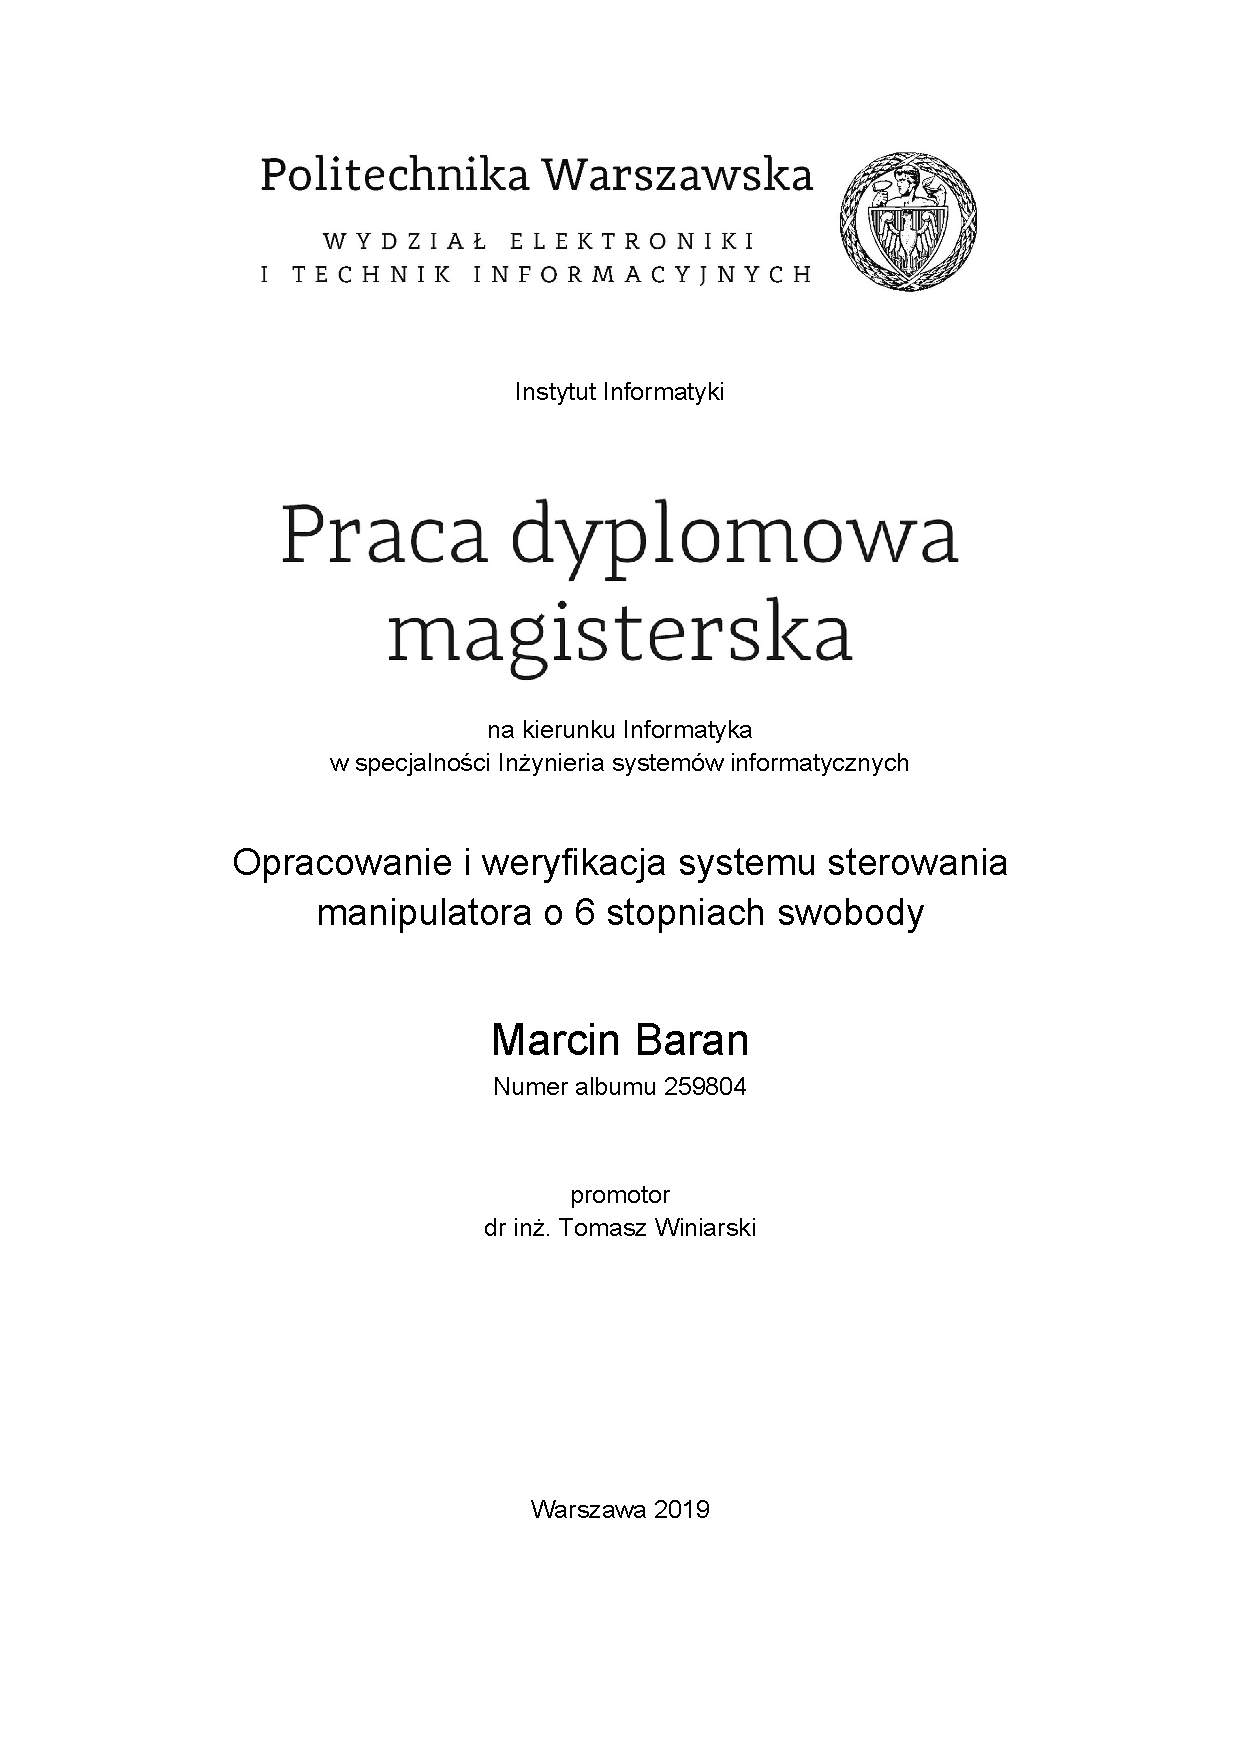
\includepdf[pages=1-2]{template/Strona_tytulowa_praca_dyplomowa_mgr_EiTI.pdf}
\setlength{\voffset}{-2.54cm}
\setlength{\hoffset}{-2.54cm}
\end{figure}
\mbox{}
\newpage
\thispagestyle{empty}
\mbox{}

%%%%%%%%%%%%%%%%%%%%%%%%%%%%%%%%%%%%%%%%
\newpage
\begin{center}
\section*{Opracowanie i weryfikacja systemu sterowania manipulatora o 6 stopniach swobody}
\end{center}

\section*{Streszczenie}
\thispagestyle{empty}
\justify
Celem pracy było opracowanie, implementacja i weryfikacja działania systemu sterującego manipulatorem antropomorficznym. Opisane zostały istniejące rozwiązania oraz narzędzia wykorzystane podczas tworzenia projektu. Sterownik robota został wykonany wykorzystując koncepcję agenta upostaciowionego. System składa się z dwóch części. Pierwszą z nich jest oprogramowanie kontrolujące wszystkie peryferia robota i jest oparte na systemie czasu rzeczywistego. Komendy sterujące ruchem manipulatora przekazywane są ze sterownika monitorującego jego stan za pomocą warstwy pośredniczącej (interfejsu sprzętowego). Dodatkowo sterownik połączony został z oprogramowaniem symulacyjnym, co pozwala na sprawdzenie jego działania w wirtualnym środowisku, bez uruchamiania rzeczywistego manipulatora. Główny kontroler robota został oparty o mikrokontroler STM32F407-VET, a program sterujący został napisany wykorzystując biblioteki Standard Peripheral Libraries (STDPeriph) oraz system czasu rzeczywistego FreeRTOS. Sterownik został przygotowany z zastosowaniem pakietu Robot Operating System (ROS) oraz środowiska symulacji Gazebo. Weryfikację systemu wykonano poprzez analizę testów ruchu robota po zadanej trajektorii do określonej pozycji.
\vspace{0.5 cm}
\\
\textit{Słowa kluczowe:}
\\
\textit{Manipulator, System Czasu Rzeczywistego, ROS, FreeRTOS, Symulacja}


%%%%%%%%%%%%%%%%%%%%%%%%%%%%%%%%%%%%%%%%
\newpage
\begin{center}
\section*{Implementation and analysis of 6 degrees of freedom robotic manipulator control system}
\end{center}

\section*{Abstract}
\thispagestyle{empty}
\justify
The aim of this thesis was to invent, implement and verify the operation of antropomorphic manipulator's control system. State of the art and technologies used in system development were discussed. The control driver was designed using an embodied agent theory. The system consists of two parts. First of them is a software managing all robot's peripherals and it is based on a real time operating system (RTOS). The manipulator's movement control commands are transfered from the driver which is monitoring the manipulator's state using hardware interface. Additionally the driver was created along with simulation software. That makes it possible to check it's performance in virtual environment, with no necessity to use actual robot. The main manipulator's controller is STM32F407-VET microchip and it's program was written using Standard Peripheral Libraries (STDPeriph) and FreeRTOS real time operating system. The control driver was prepared based on Robot Operating System (ROS) software and Gazebo simulation environment. The system's verification was done by analysing robot's tests of movement along specified trajectory to given position.
\vspace{0.5 cm}
\\
\textit{Keywords:}
\\
\textit{Manipulator, Real Time Operating System, ROS, FreeRTOS, Simulation}

%%%%%%%%%%%%%%%%%%%%%%%%%%%%%%%%%%%%%%%%
\newpage
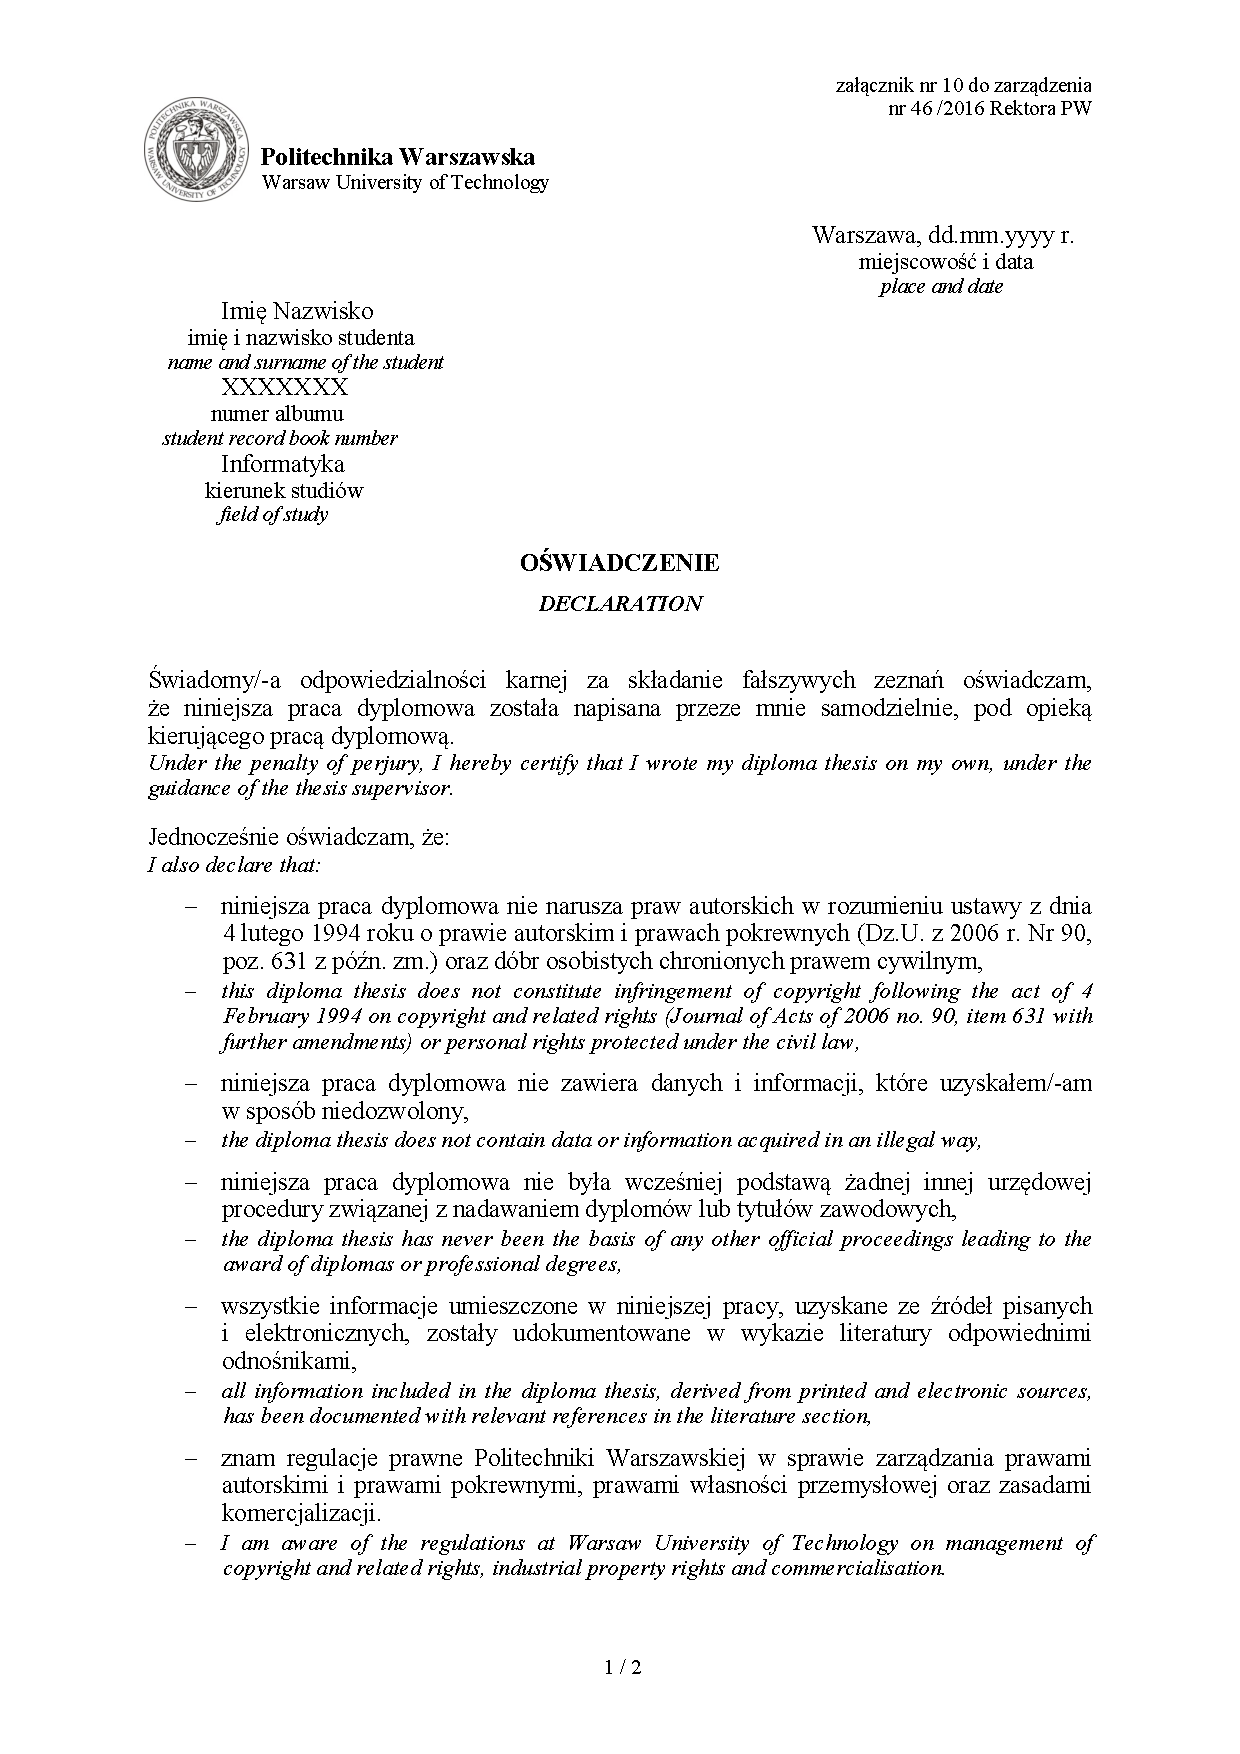
\includepdf[pages=1-2]{template/Oswiadczenie_autora_pracy_dyplomowej_w_jezyku_angielskim.pdf}

%%%%%%%%%%%%%%%%%%%%%%%%%%%%%%%%%%%%%%%%

\tableofcontents

%%%%%%%%%%%%%%%%%%%%%%%%%%%%%%%%%%%%%%%%
\newpage
\justify

% Początek treści	
\vspace*{1.5 cm}
\section{Wprowadzenie}
\vspace{1.5 cm}

W latach 1960-1990 robotyka skupiona była głównie na wykorzystaniu robotów do pracy w przemyśle i automatyzacji procesów produkcyjnych. Dzięki ciągłemu rozwojowi w tym polu roboty stały się wszechobecne. W ostatnich kilkudziesięciu latach można zaobserwować rosnące zastosowanie robotów w domenach wykraczających poza ramy samego przemysłu. Międzynarodowa Organizacja Normalizacyjna (ISO) definiuje roboty usługowe jako roboty wykonujące autonomicznie lub półautonomicznie użyteczne zadania dla ludzi lub sprzętu z wyłączeniem zastosowań do automatyzacji procesów \cite{isodef}. Przykładami takiego wykorzystania mogą być roboty medyczne, sprzątające, czy pomagające osobom starszym. Wiele z tych zastosowań wymaga bezpośredniej interakcji z ludźmi i otoczeniem w precyzyjny i bezpieczny sposób. Stąd przed wprowadzeniem takich rozwiązań do użytku i kontaktu z otoczeniem powinny one być dokładnie sprawdzone i przetestowane w środowisku symulacyjnym. 

\subsection{Motywacja}

Celem pracy magisterskiej jest opracowanie systemu sterowania do autorskiego projektu manipulatora o 6 stopniach swobody. Stworzenie systemu do kontroli ruchu takiego robota wiąże się z kilkoma wymaganiami. Głównym z nich jest bezpieczeństwo użytkownika, a także otoczenia. Z tego względu użytkownik powinien móc sprawdzić poprawność zadanego ruchu przed wykonaniem go na urządzeniu. Ewentualnie występujące błędy mogą generować duże koszty i stanowić zagrożenie. Ponadto oprogramowanie samego robota, które bezpośrednio kontroluje jego napędami, a także odbiera komendy ruchu i wysyła dane o aktualnym stanie powinno być zabezpieczone w przypadku pojawienia się sytuacji zapobiegającej poprawnemu działaniu urządzenia. 

Ze względu na wyżej wymienione wymagania opracowany system sterujący powinien pozwalać na weryfikację sterownika poza urządzeniem, a także na możliwie szybkie przeniesienie jego działania na urządzenie. Symulacja rzeczywistego robota pozwala na testy i analizę jakości sterowania i poprawności wykonywanych zadań w środowisku wirtualnym. Następnie zadania te mogą zostać wykonane bezpośrednio na robocie dzięki połączeniu programu symulacyjnego ze sterownikiem urządzenia wykorzystując w tym celu odpowiednio przygotowany interfejs sprzętowy. Zastosowanie systemu czasu rzeczywistego do kontrolowania napędów manipulatora, odczytywania danych z sensorów i komunikowania się z interfejsem sprzętowym sterownika pozwala na wykonanie każdego z tych zadań w zdefiniowanym i najkrótszym czasie, a w przypadku wystąpienia opóźnienia lub błędu zapewnia bezpieczne jego zatrzymanie. Opisany system w znaczącym stopniu ułatwia programowanie, testowanie i wykonywanie ruchów robota. Składa się on z zadajnika (myszki 3D pozwalającej na ręczne zadawanie ruchu robota), aplikacji symulacyjnej i sterującej na komputer PC oraz oprogramowania na mikrokontroler z serii STM32F4.

Konstrukcja i oprogramowanie manipulatora szeregowego jest częścią projektu łazika marsjańskiego Koła Naukowego Robotyków działającego na Wydziale Mechanicznym Energetyki i Lotnictwa Politechniki Warszawskiej.

\subsection{Plan pracy}

Dokument ten stanowi raport z przeprowadzonej pracy magisterskiej. Składa się on z~następujących części:
\begin{itemize}
\item rozdział 2 zawiera wprowadzenie teoretyczne do dziedziny kinematyki mechanizmów wieloczłonowych; zostały w nim opisane zadania proste i odwrotne kinematyki manipulatorów oraz notacja Denavita-Hartenberga użyta do opisu konfiguracji manipulatora,
\item rozdział 3 opisuje konstrukcje i technologie użyte w projekcie autorskiego manipulatora szeregowego,
\item rozdział 4 przedstawia architekturę oprogramowania wykorzystując koncepcję agenta upostaciowionego i język opisu sprzętowego SysML,
\item rozdział 5 ukazuje działanie oprogramowania kontrolera robota opartego na systemie czasu rzeczywistego FreeRTOS,
\item rozdział 6 przedstawia działanie sterownika i oprogramowania symulacyjnego stworzonego z pomocą pakietu ROS oraz środowiska Gazebo,
\item rozdział 7 stanowi szczegółowy opis przeprowadzonych testów ruchu manipulatora w środowisku symulacyjnym Gazebo,
\item rozdział 8 opisuje wyniki zebrane podczas testów oraz analizę dokładności wykonywania zadanego sterowania,
\item rozdział 9 poświęcony jest podsumowaniu pracy.  
\end{itemize} 

\subsection{Analiza trendów}

Oprogramowanie sterujące każdego robota jest rozwijane mając na uwadze to, że powinno być w stanie zapewnić jego użytkownikowi zaimplementowanie wykonywanego przez robota zadania w możliwie prosty sposób. Aby było to możliwe system sterujący powinien być przygotowany tak, aby pozwalał na:

\begin{itemize}
\item zdefiniowanie prędkości poszczególnych napędów
\item zdefiniowanie pozycji chwytaka/narzędzia
\item zaprogramowanie robota, by podążał wyznaczoną ścieżką
\item zaprogramowanie robota, by wykonywał określone zadanie
\end{itemize}

Zieliński w swoim artykule \cite{ramowezielinski} wskazuje na ewolucje podejścia przy tworzeniu oprogramowania sterującego robotami jakie nadeszło wraz z rosnącym rozwojem robotyki i tym samym zwiększaniem liczby rodzajów stosowanych konstrukcji. W rozwiązaniach przemysłowych głównymi metodami programowania ruchu są:

\begin{itemize}
\item programowanie online (nietekstowe)- polega na tym, że operator przesuwa robota do wymaganych pozycji, które są zapamiętywane, a później odtwarzane
\item programowanie offline (tekstowe)- polega na wykorzystaniu specjalnie przygotowanego języka komend i struktur do definiowania rodzaju i punktów docelowych ruchu robota
\end{itemize}

Rozszerzenie programowania nietekstowego o formę programowania offline spowodowało powstanie hybrydowej metody programowania robotów, która jest dziś szeroko stosowana w przemyśle. Jednym z przykładów takiego rozwiązania jest KUKA Robot Language (KRL) \cite{kukawebsite} dedykowany do robotów firmy KUKA. Jednakże ze względu na pojawiające się nowe rodzaje robotów ta metoda wymaga ciągłej zmiany języków programowania, a także ich interpreterów.

W książce Kozłowskiego i innych \cite{systemkozlowski} w rozdziale poświęconym systemom programowania robotów autorzy wskazują uwagę na fakt, że w pracach badawczych dotyczących algorytmów sterowania i planowania trajektorii często używane są roboty przemysłowe. Dużą przeszkodą w prowadzeniu takich prac jest zamknięta konstrukcja sterownika robota przemysłowego. W dodatku projektowane są one do wykonywania określonych i powtarzalnych zadań, stąd są mało przydatne w celach badawczych. Z tego względu autorzy zaproponowali połączenie robota posiadającego własny sterownik z komputerem PC stosując jedno z dwóch rozwiązań:

\begin{itemize}
\item wykorzystując robota z interfejsem sieciowym do komunikacji
\item własnoręcznie definiując i implementując interfejs komunikacji z urządzeniem
\end{itemize} 

Przedstawione zostały oba rozwiązania. Autorzy stworzyli dwa stanowiska badawcze: jedno z nich oparte na manipulatorach przemysłowych Sta{\"u}bli RX60 z własnym interfejsem sieciowym, drugie na manipulatorze produkcji polskiej IRp-6 ze specjalnie do niego stworzonym interfejsem komunikacyjnym. W ten sposób udało się uzyskać uniwersalny system programowania bez ingerencji w oprogramowanie producenta składający się z trzech części (rysunek \ref{fig:system_scheme}):

\begin{itemize}
\item sterownika robota
\item urządzeń pomiarowych
\item komputera nadrzędnego
\end{itemize}

\begin{figure}[hbt!]
\centering
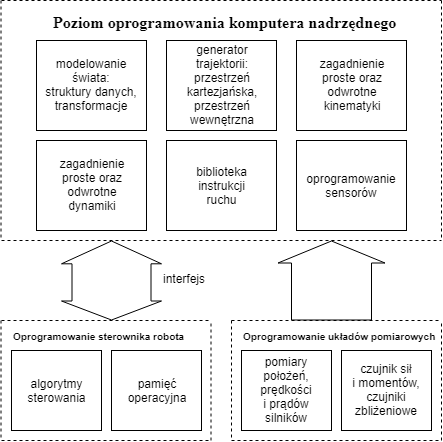
\includegraphics[width=0.8\linewidth]{images/system_scheme.png}
\caption{Schemat stworzonego systemu programowania\textit{ (Źródło: \cite{systemkozlowski}) } }
\label{fig:system_scheme}
\end{figure}

Autorzy dodatkowo opracowali od podstaw oprogramowanie komputera nadrzędnego, które pozwoliło na rozszerzenie możliwości sterowania robotem poprzez napisanie własnych programów sterujących (w uniwersalnych językach wysokiego poziomu, takich jak C++). Taka architektura systemu daje większe możliwości względem specjalizowanych języków programowania wspomnianych wcześniej. Jednakże stworzenie programów sterujących od podstaw zajmuje dużo czasu. Z tego względu rozsądnym byłoby dołączenie dodatkowych, uniwersalnych bibliotek z szablonami potrzebnych funkcjonalności i dostosowaniu ich do badanego robota. Takim rozwiązaniem są programowe struktury ramowe (ang. frameworks).

W dalszej części artykułu \cite{ramowezielinski} autor opisuje programowe struktury ramowe jako bibliotekę oraz wzorce jej wykorzystania. Użytkownik może ją dostosować do swojego urządzenia używając dobrze udokumentowane szablony oraz dostarczone z nią narzędzia, do których zaliczyć można symulatory czy debuggery. Dodatkowo autor wskazuje, że wykorzystanie programowych struktur ramowych w robotyce doprowadziło do zaniku podziału na oprogramowanie sterujące sprzętem, interpreter języka programowania robota i program użytkowy. Nie ma potrzeby użycia specjalnego interpretera z tego względu, że program użytkowy jest tworzony w tym samym języku co oprogramowanie sterujące. To rozwiązanie pozwala na znaczne przyspieszenie tworzenia oprogramowania, a także na łatwe dołączenie dodatkowych funkcjonalności systemu.

Jednym z przykładów takiej struktury jest ROS \cite{rosdesc}, który jest jednym z najpopularniejszych i najbardziej zaawansowanych narzędzi do tworzenia sterowników robotycznych. O jego popularności świadczyć może duża liczba literatury badawczej, w której pomocny był ten pakiet. Kilka pozycji zostało wymienione poniżej:

\begin{itemize}
\item \textit{Sterowanie predykcyjne z wykorzystaniem wizji w zadaniu śledzenia ścieżki przez robota mobilnego\cite{thesismeyer}}: 

Praca przedstawia badanie wykorzystania algorytmów sterowania predykcyjnego do zadania śledzenia ścieżki. Zadanie wykonywane jest przez robota mobilnego klasy 2.0 na podstawie danych z kamery zamontowanej na robocie albo umieszczonej nad trasą, którą podążać ma robot. W pracy wykorzystano bibliotekę OpenCV do przetwarzania obrazu oraz środowisko MATLAB do implementacji algorytmów sterowania. System sterowania podzielono zgodnie z poniższym schematem:

\begin{figure}[hbt!]
\centering
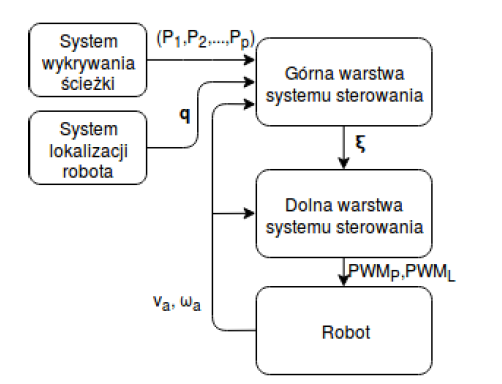
\includegraphics[width=0.8\linewidth]{images/mobile_robot_system.png}
\caption{Struktura systemu sterowania robotem mobilnym\textit{ (Źródło: \cite{thesismeyer}) } }
\label{fig:mobile_robot_scheme}
\end{figure}

Ze względu na to, że system składa się z wielu równolegle działających procesów na trzech różnych platformach (komputer stacjonarny, komputer jednopłytkowy Raspberry Pi, mikrokontroler) autor wykorzystał pakiet ROS do komunikacji pomiędzy zadaniami oraz użył go do rejestracji i wizualizacji danych. ROS bardzo dobrze nadaje się do implementacji komunikujących się procesów. Poszczególne procesy są w nim odzwierciedlane jako węzły (ang. \textit{nodes}), które komunikują się poprzez tematy (ang. \textit{topics}).

\item \textit{System robotyczny chwytający obiekty \cite{thesiskarbarczyk}}:

Celem pracy było stworzenie systemu robotycznego opartego o manipulator IRp-6, który umożliwiałby chwytanie obiektu. Zadanie chwytania wykonywane było stosując obraz z kamery 2D zamontowanej w kiści robota oraz znając model chwytanego przedmiotu. W tym przypadku system ROS został użyty w połączeniu z systemem IRPOS (IRp-6 ). Służy on do sterowania dwoma robotami IRp-6 (o nazwach \textit{Track} i \textit{Postument}) i zawiera wiele gotowych rozwiązań ułatwiających wykonywanie skomplikowanych trajektorii ruchu ramienia robota. Dodatkowo do przetwarzania obrazu użyto biblioteki OpenCV oraz struktury ramowej DisCODe do przetwarzania danych uzyskanych z kamery. Wykorzystanie systemu ROS do komunikacji i procesowania wszystkich zadań daje możliwość dalszego rozwoju projektu poprzez dodanie kolejnych węzłów wykonujących nowe zadania. Ponadto różnorodność użytych komponentów i bibliotek wskazuje na bardzo elastyczną inkorporacje gotowych rozwiązań do systemu robotycznego opartego o ROS.

\item \textit{Development of autonomous driving using Robot Operating System \cite{thesiszivkovic})}:

Praca skupia się na opisie wykorzystania ROS do stworzenia oprogramowania przeznaczonego do autonomicznej jazdy. W celu weryfikacji zaimplementowanych rozwiązań stworzony system zastosowany jest w zdalnie sterowanym pojeździe wyposażonym w jednopłytkowy komputer pojazdu Raspberry Pi 3, płytkę z mikrokontrolerem Arduino Uno do sterowania silnikami oraz czujniki takie jak: kamera 2D, ultradźwiękowe czujniki odległości i IMU (ang. \textit{Intertial Measurement Unit}). W tym projekcie architektura systemu została całkowicie oparta o pakiet ROS zainstalowany na komputerze pojazdu z systemem operacyjnym Ubuntu 16.04.

\begin{figure}[hbt!]
\centering
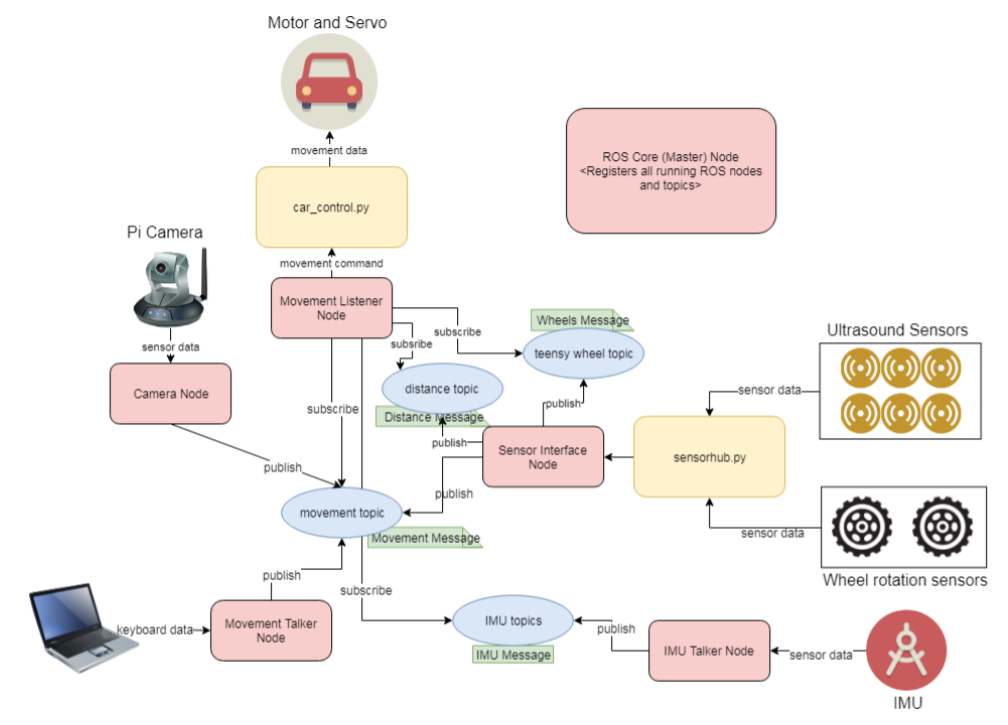
\includegraphics[width=0.8\linewidth]{images/autonomous_car_system.png}
\caption{Struktura systemu sterowania autonomicznym pojazdem RC\textit{ (Źródło: \cite{thesiszivkovic}) } }
\label{fig:autonomous_car_scheme}
\end{figure}

Zgodnie z grafiką \ref{fig:autonomous_car_scheme} operacje każdego z elementów systemu (komunikacja zdalna z użytkownikiem, akwizycja oraz obróbka obrazu z kamery, czujników ultradźwiękowych i IMU, sterowanie silnikami) odbywa się w oddzielnym węźle ROS (oznaczone na czerwono). Przesyłanie danych odbywa się za pomocą zdefiniowanych tematów (oznaczone na niebiesko) i na podstawie tych danych sterowane są silniki pojazdu.

Autor wskazuje na zalety systemu ROS, takie jak możliwość tworzenia modułowego oprogramowania oraz szeroką dostępność gotowych bibliotek czujników i narzędzi symulacyjnych. W pracy użyto symulatora Gazebo przystosowanego do współpracy z ROS w celu przetestowania systemu sterowania pojazdem. 

Oprócz tego zauważone zostają wady takie jak istnienie pojedynczego punktu awarii, jakim jest zbiór węzłów \textit{roscore}. Są one wymagane w celu komunikacji pomiędzy uruchomionymi procesami (węzeł ROS Master). Ponadto autor wskazuje, że komunikacja w sieci ROS nie jest zabezpieczona, co może stanowić zagrożenie bezpieczeństwa systemu. Obie te niedogodności są rozwiązywane w ramach powstania nowej wersji oprogramowania ROS (ROS version 2).

\end{itemize}

Szeroka gama gotowych modułów dodatkowych (takich jak symulator Gazebo), możliwość łatwego rozszerzania funkcjonalności systemu sterowania opartego o ROS oraz łatwość w dostosowaniu gotowych bibliotek do współpracy z pakietem zdecydowały o użyciu tego pakietu w niniejszej pracy. 

%%%%%%%%%%%%%%%%%%%%%%%%%%%%%%%%%%%%%%%%
\newpage
\vspace*{1.5 cm}
\section{Kinematyka mechanizmów wieloczłonowych}
\vspace{1.5 cm}
Niniejszy rozdział przedstawia podstawy teoretyczne sterowania manipulatorem o strukturze szeregowej. Manipulator jest definiowany jako mechanizm wieloczłonowy, czyli łancuch sztywnych członów połączonych ruchomymi przegubami, które pozwalają na ruch względny członów. Istnieje kilka róznych typów przegubów, jednakże najczęściej stosowanymi są tylko dwa:

\begin{itemize}
\item obrotowy - pozwalajacy na obrót członu wzgledem tylko jednej osi
\item postępowy - pozwalający na ruch postępowy członu tylko w jednym kierunku
\end{itemize}

Podstawowym parametrem charakteryzującym manipulator jest liczba stopni swobody, która określa najmniejszą liczbę współrzędnych jednoznacznie opisujacą jego konfigurację (połozenie i orientację w przestrzeni każdego członu). Ze względu na to, że najczęściej stosowane typy przegubów pozwalają na ruch postępowy albo obrotowy względem jednej osi, liczba stopni swobody
często równa jest liczbie przegubów. Aby koncówka manipulatora (efektor) mogła uzyskać jednoznacznie zadane połozenie i orientację w przestrzeni trójwymiarowej potrzebna jest znajomość 6 współrzędnych. Z tego wzgledu najczęściej stosowane są konstrukcje manipulatorów o 6 stopniach swobody.

\begin{figure}[H]
\centering
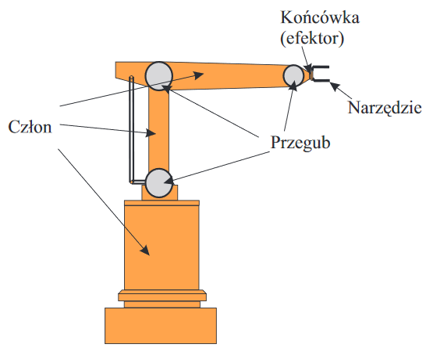
\includegraphics[width=0.6\linewidth]{images/manipulator_scheme.png}
\caption{Konstrukcja manipulatora szeregowego\textit{ (Źródło: \cite{lectures}) } }
\label{fig:manipulator_scheme}
\end{figure}

Do poprawnego sterowania manipulatorem robotycznym potrzebna jest znajomość połozenia i prędkości poszczególnych jego członów względem bazowego, nieruchomego układu współrzędnych, który nazywany jest układem globalnym. W tym celu dla każdego członu sztywnego definiuje sie związany z nim lokalny układ współrzędnych. Wtedy położenie kazdego członu można określić jako połozenie układu lokalnego wzgledem globalnego. Podstawowymi operacjami stosowanymi przy opisie kinematyki mechanizmów wieloczłonowych są rotacja i translacja o wektor. Pozwalają one na zdefiniowanie wektora przesunięcia oraz macierzy rotacji układu lokalnego
względem układu globalnego (rysunek \ref{fig:kinematic_scheme}).

\begin{figure}[hbt!]
\centering
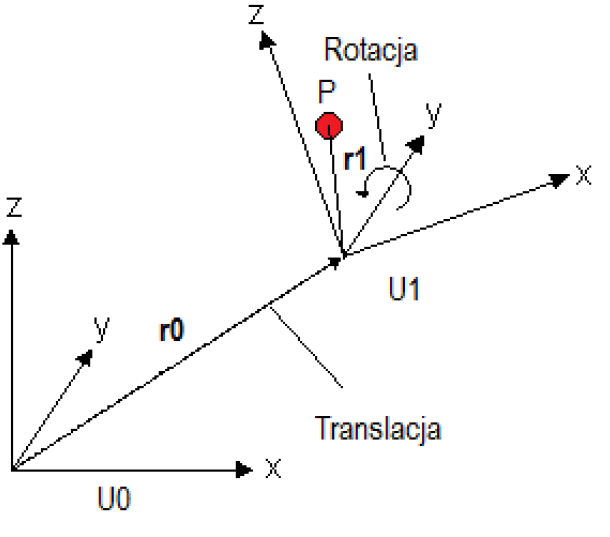
\includegraphics[width=0.6\linewidth]{images/kinematic_scheme.png}
\caption{Położenie członu P i związanego z nim układu $U_1$ opisane względem globalnego układu $U_0$ }
\label{fig:kinematic_scheme}
\end{figure}

Znając macierz rotacji $\bm{R}$, wektor translacji $\bm{r_0}$ układu lokalnego $U_1$ względem globalnego $U_0$ oraz wektor translacji członu $P$ względem układu lokalnego $U_1$ możemy wyznaczyć połozenie członu $P$ względem układu globalnego $U_0$:

\begin{equation}  \label{eq:1} 
\bm{r} = \bm{r_0} + \bm{R} \bm{r_1}
\end{equation}

Dodatkowo dla ułatwienia zapisu równań \ref{eq:1} wprowadzono pojęcie macierzy transformacji \cite{systemkozlowski} pomiędzy układem $i-1$, a układem $i$. Jest to macierz 4x4, która tworzona jest na podstawie macierzy rotacji (3x3) oraz wektora translacji (3x1) i przedstawia się następująco:

\begin{equation} \label{eq:2}
\bm{^{i-1}_{i}T} = \begin{bmatrix} 
				   \bm{R_{3x3}} & \bm{r_{i-1,3x1}} \\
				   0_{1x3} & 1 
				   \end{bmatrix}
\end{equation}

Wtedy odnosząc się do rysunku \ref{fig:kinematic_scheme} położenie członu $P$ opisane względem globalnego układu $U_0$ można opisać jako:

\begin{equation} \label{eq:3}
\begin{bmatrix}
\bm{r} \\
1
\end{bmatrix} = \bm{^{0}_{1}T}\begin{bmatrix}
								\bm{r_0} \\
								1
								\end{bmatrix}
\end{equation}

\subsection{Notacja Denavita-Hartenberga}

Powszechną metodą opisu położenia poszczególnych ogniw dla manipulatora posiadającego jedynie pary obrotowe i postępowe jest notacja Denavita-Hartenberga, w której każdemu członowi przyporządkowane są cztery wartości \cite{systemkozlowski}:

\begin{itemize}
\item $a_{i-1}$ - długość $i-1$ ogniwa, mierzona jako odległość między osiami przegubów $i-1$ oraz~$i$,
\item $\alpha_{i-1}$ - kąt skręcenia $i-1$ ogniwa prawoskrętnie wokół $a_i$, mierzony jako kąt między osiami przegubów $i$ oraz $(i+1)$,
\item $d_i$ - odległość mierzoną wzdłuż osi $i$-tego przegubu między $a_{i-1}$ i $a_i$,
\item $\theta_i$ - kąt między $a_{i-1}$ i $a_i$, określony prawoskrętnie wokół osi $i$-tego przegubu.
\end{itemize}

Metoda zakłada również, że osie ortogonalnego układu współrzędnych, związanego z $i$-tym ogniwem są skierowane następująco \cite{systemkozlowski}:

\begin{itemize}
\item $z_i$ pokrywa się z osią $i$-tego przegubu,
\item $x_i$ jest prostopadła do osi $z_i$ oraz $z_{i+1}$ i jest skierowana od przegubu $i$ do $i+1$,
\item $y_i$ uzupełnia prawoskrętny układ współrzędnych.
\end{itemize}

Ze względu na przyjęte powyżej założenia notacja wymaga znajomości czterech parametrów do określenia wzajemnego położenia układów zamiast sześciu.

\subsection{Zadanie proste i odwrotne kinematyki}

W trakcie pracy robota jego układ sterowania musi być w stanie określić położenie końcówki na podstawie położenia każdego z jego napędów (a tym samym członów). Ponadto chcąc zmienić położenie końcówki należy wiedzieć w jaki sposób powinny być ułożone poszczególne człony, aby daną pozycję osiągnąć. Z tego względu wymagane jest rozwiązanie zadania prostego i odwrotnego kinematyki dla zadanego robota.

\paragraph{Zadanie proste kinematyki}polega na tym, aby wyznaczyć współrzędne zewnętrzne manipulatora (wpółrzędne końcówki), kiedy dane są współrzędne wewnętrzne (każdego z członów). Sprowadza się więc ono zatem do znalezienia macierzy transformacji $\bm{^{0}_{n}T}$ (gdzie $n$ to liczba stopni swobody) i obliczenia wektora współrzędnych $\bm{r}$, tak jak pokazano to w przykładzie z rysunku \ref{fig:kinematic_scheme}:

\begin{equation} \label{eq:4}
\begin{bmatrix}
\bm{r} \\
1
\end{bmatrix} = \bm{^{0}_{n}T}\begin{bmatrix}
								\bm{s} \\
								1
								\end{bmatrix}
\end{equation}, przy czym $\bm{s}$ to współrzędne końcówki w układzie związanym z ostatnim stopniem swobody.

\paragraph{Zadanie odwrotne kinematyki}służy obliczeniu współrzędnych członów znając położenie i orientację końcówki robota. Dla manipulatorów szeregowych wiążę się z rozwiązaniem nieliniowego układu równań i może nie mieć jednoznacznego rozwiązania (na przykład gdy manipulator ma więcej niż 6 stopni swobody). Ze względu na niekiedy trudne znalezienie rozwiązań analitycznych zadania odwrotnego dla skomplikowanych konstrukcji do jego rozwiązania stosuje się metody numeryczne. Przyjmując za szukany wektor współrzędnych wewnętrznych manipulatora $\bm{q}$, taki że:

\begin{equation} \label{eq:5}
\bm{q} = [ q_1  q_2  ...  q_n ]^T
\end{equation}

można przedstawić rozwiązywany układ równań jako:

\begin{equation} \label{eq:6}
\bm{\phi}(\bm{q}) = \begin{bmatrix}
					\phi^1(\bm{q}) \\
					\phi^2(\bm{q}) \\
					... \\
					\phi^n(\bm{q}) \\
					\end{bmatrix} = 0_{nx1}
\end{equation}

Mając postawiony problem w tej postaci można rozwiązać go stosując na przykład metodę Newtona-Rhapsona. Metody numeryczne są często wykorzystywane do rozwiązywania zadania odwrotnego w oprogramowaniu symulacyjnym (pakiet ROS także posiada biblioteki na to pozwalające).

%%%%%%%%%%%%%%%%%%%%%%%%%%%%%%%%%%%%%%%%
\newpage
\vspace*{1.5 cm}
\section{Opis narzędzi}
\vspace{1.5 cm}

\subsection{Sprzęt}

\subsubsection{Manipulator}
System sterowania opracowywany jest do autorskiej konstrukcji manipulatora o 6 stopniach swobody. Głównym założeniem robota było jego wykorzystanie jako ramię operacyjne dla prototypu łazika marsjańskiego przeznaczonego do startu w zawodach URC 2018. Manipulator przedstawiony jest na zdjęciu poniżej \ref{fig:manipulator_photo}:

\begin{figure}[hbt!]
\centering
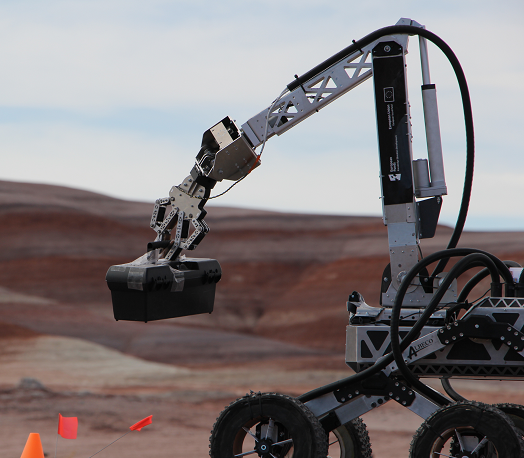
\includegraphics[width=0.5\linewidth]{images/manipulator_photo.png}
\caption{Zaprojektowany manipulator wykonujący zadanie konkursowe }
\label{fig:manipulator_photo}
\end{figure}

Konstrukcja stworzona była biorąc pod uwagę regulaminowe wymagania i ograniczenia konkursowe \cite{competitionwebsite}:

\begin{itemize}
\item lekka konstrukcja o masie 13 kg
\item udźwig do 5 kg
\item zasięg maksymalny 1.2 m
\item moźliwość wykonywania precyzyjnych zadań, takich jak odkręcanie zaworów, przełączanie przycisków, unoszenie przedmiotów o nieregularnym kształcie
\end{itemize}

Skonstruowany manipulator wykorzystuje przeguby obrotowe do poruszania każdym stopniem swobody. Ze wzgledu na powyższe wymagania mechanizm został złożony wykorzystując elementy z giętej blachy aluminiowej oraz elementy wytworzone metodą druku 3D. Jako napędów do poruszania przegubów użyto 3 silników DC, 1 siłownika i 2 serwomechanizmów Dynamixel RX-64 \cite{servo}. Manipulator zasilany jest napieciem 12 V. Sterowany jest za pomocą mikrokontrolera STM32F407-VET. Informacje o aktualnej prędkości i pozycji poszczególnych przegubów uzyskiwane są wykorzystując odczyty z enkoderów magnetycznych. Robot wyposażony jest w 2 interfejsy komunikacyjne: UART oraz CAN. Ponadto do komunikacji z serwomechanizmami wykorzystywany jest interfejs RS-485. Schemat elektroniczny manipulatora przedstawia poniższy diagram:



Konfigurację poszczególnych członów manipulatora opisano wykorzystując następujące parametry Denavita-Hartenberga (zgodnie z ustalonymi układami współrzędnych każdego z członów):

%TODO : Uzupełnić parametry!
\begin{table}[htb!]
\begin{center}
\caption{Parametry Denavita-Hartenberga manipulatora}
\begin{tabular}{ | c | c | c | c | c |}
\hline
 i & $\alpha_{i-1} [rad]$ & $a_{i-1} [m]$ & $\delta_{i} [m]$ & $\theta_{i} [rad]$ \\ 
\hline
 1 & $\pi/2$ & 0 & 0.13 & $\theta_{1}$ \\ 
\hline
 2 & $\pi/2$ & 0 & 0.0705 & $\theta_{2} + \pi/2$ \\
\hline
 3 & c & c & c & $\theta_{3}$ \\
\hline
 4 & c & c & c & $\theta_{4}$ \\ 
\hline
 5 & c & c & c & $\theta_{5}$ \\
\hline
 6 & c & c & c & $\theta_{6}$ \\
 \hline
\end{tabular}
\end{center}
\end{table}

%TODO Rysunek konfiguracji manipulatora!
\subsubsection{Mysz 3D}

Jako zadajnik ruchu wykorzystywana jest mysz 3D Magellan Space Mouse Plus \cite{spacemouse} (rysunek \ref{fig:mouse}). Pozwala ona na wygodne ręczne sterowanie manipulatorem z wykorzystaniem możliwości ruchu (translacji i obrotu) w 3 niezależnych osiach. Komunikacja z komputerem odbywa się poprzez interfejs szeregowy RS-232.

\begin{figure}[hbt!]
\centering
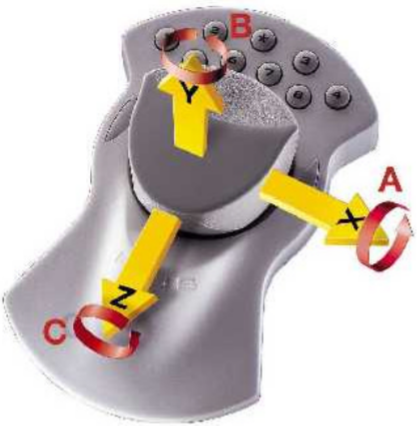
\includegraphics[width=0.4\linewidth]{images/mouse.png}
\caption{Mysz 3D Magellan Space Mouse Plus\textit{ (Źródło: \cite{spacemouse}) } }
\label{fig:mouse}
\end{figure}

\subsection{Oprogramowanie}

\subsubsection{SysML}

SysML (ang. System Modeling Language)\cite{sysml} jest jedną z metod graficznego opisu specyfikacji oraz implementacji systemów. Jest to język modelowania, który powstał jako modyfikacja i rozbudowa standardu UML (ang. Unified Modeling Language). Zawiera on 9 typów diagramów podzielonych na 3 rodzaje: 
\begin{itemize}
\item diagramy zachowań,
\item diagramy wymagań systemowych,
\item diagramy struktury.
\end{itemize}

W pracy wykorzystano diagram przypadków użycia (ang. Use Case Diagram), diagram maszyny stanowej (ang. State Machine Diagram), diagram bloków wewnętrznych (ang. Internal Block Diagram), rozszerzony diagram czynności (ang. Activity Diagram) oraz diagram sekwencji (ang. Sequence Diagram).

\subsubsection{Koncepcja agenta upostaciowionego}

W pracy wykorzystano również koncepcje agenta upostaciowionego \cite{embodiedagent} w celu opisu systemu. Metodyka ta zakłada podział systemu na grupę agentów utrzymujących ze sobą komunikację. Ogólny schemat przedstawiający agenta upostaciowionego przedstawiony jest na rysunku \ref{fig:embodied_agent}.

\begin{figure}[hbt!]
\centering
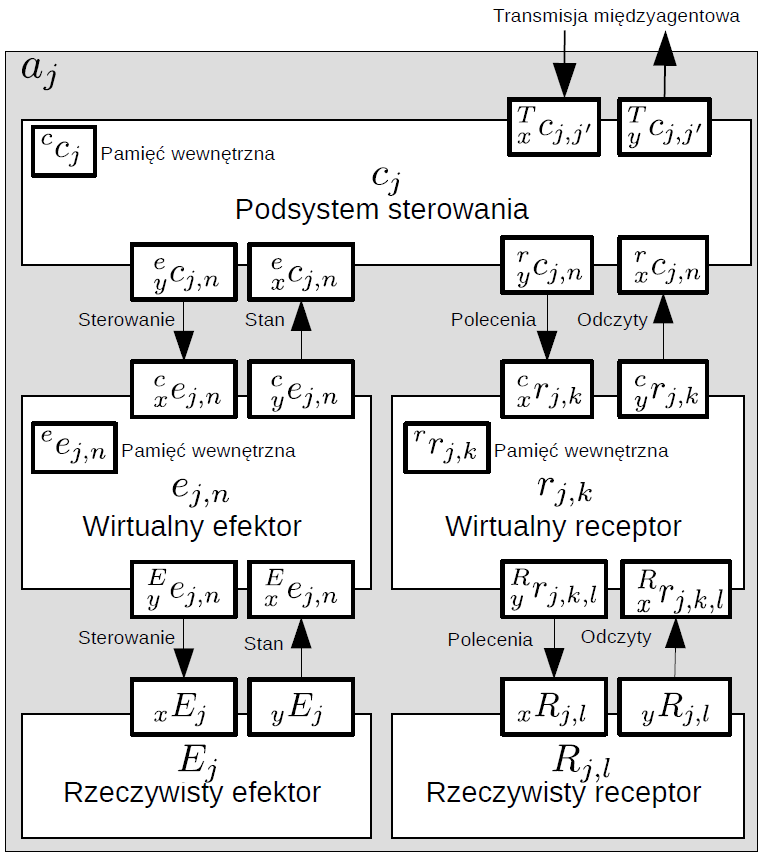
\includegraphics[width=0.6\linewidth]{images/embodied_agent.png}
\caption{Schemat agenta upostaciowionego \textit{ (Źródło: TODO) } }
\label{fig:embodied_agent}
\end{figure}

Każdy agent (oznaczony na rysunku \ref{fig:embodied_agent} jako $a_j$) posiada dokładnie jeden podsystem sterowania i może posiadać po kilka wirtualnych oraz rzeczywistych receptorów i efektorów, które opisane są poniżej:

\begin{itemize}
\item podsystem sterowania ($c_j$) - wykonuje zadanie zgodne z aktualnym stanem na podstawie danych z wirtualnych efektorów i receptorów poprzez wydawane im komendy; ponadto podsystem sterowania odpowiada za komunikację z innymi agentami w systemie;
\item rzeczywisty efektor ($E_j$) - to fizyczne części, którymi agent może oddziaływać na środowisko zewnętrzne (w przypadku manipulatora to silniki do poruszania każdym z jego członów);
\item rzeczywisty receptor ($R_{j,l}$) - są to czujniki dające wiedzę o stanie środowiska zewnętrznego
\item wirtualny efektor ($e_{j,n}$) - jest to abstrakcyjna warstwa pośrednicząca między rzeczywistym efektorem, a podsystemem sterowania, jej zadaniem jest modyfikowanie komend sterujących i danych o stanie rzeczywistego efektora (przykładowo przelicza zadaną komendę prędkości z wartości wyrażonej w rad/s do wartości PWM na silnikach);
\item wirtualny receptor ($r_{j,k}$) - tak jak wirtualny efektor pośredniczy w komunikacji pomiędzy rzeczywistym receptorem, a podsystemem sterowania (na przykład poprzez przeliczanie odczytów czujników).
\end{itemize}

\subsubsection{ROS}

ROS (Robot Operating System) \cite{rosdesc} jest to ogólnodostępna programowa struktura ramowa służąca
do tworzenia i rozwijania oprogramowania dla robotów. Zawiera biblioteki i narzędzia dostarczające gotowe sterowniki urządzeń i/lub rozwiązania przydatne do sterowania, testowania i symulowania pracy robota. ROS wspiera jezyki programowania C++ i Python. Program stworzony stosując pakiet ROS składa się z takich elementów jak:
\begin{itemize}
\item Węzły (ang. nodes) – pojedyncze procesy obliczeniowe, z których każdy odpowiada za pewną funkcjonalność. Węzły mogą komunikować się ze sobą za pomocą tematów (ang. topics);
\item Zarządca (ang. master) - jest to proces odpowiedzialny za rejestrację i obserwacje węzłów w sieci. Dzięki niemu możliwa jest odszukanie się dwóch węzłów i komunikacja między nimi. Stąd do poprawnego działania wymagane jest uruchomienie węzła zarządcy. Ponadto zarządca udostępnia do użytku serwer parametrów;
\item Wiadomości (ang. messages) – zdefiniowane przez użytkownika struktury danych, które mogą być przesyłane pomiędzy węzłami wykorzystując tematy;
\item Tematy (ang. topics) – nazwane porty komunikacji pomiędzy węzłami, które mogą publikować lub subskrybować się na wiadomości nadchodzące do tematu;
\item Usługi (ang. services) – typ komunikacji pytanie - odpowiedź. Pozwala na zdalne wywołanie procedury. Usługi mogą być blokujące lub nieblokujące
\item Serwer parametrów (ang. parameter server ) - służy do przechowywania danych, do których odnosić może się każdy węzeł za pomocą klucza.
\end{itemize}

Przykładowy schemat połączeń/komunikacji pomiędzy węzłami w ROS przedstawia poniższy diagram:

\begin{figure}[H]
\centering
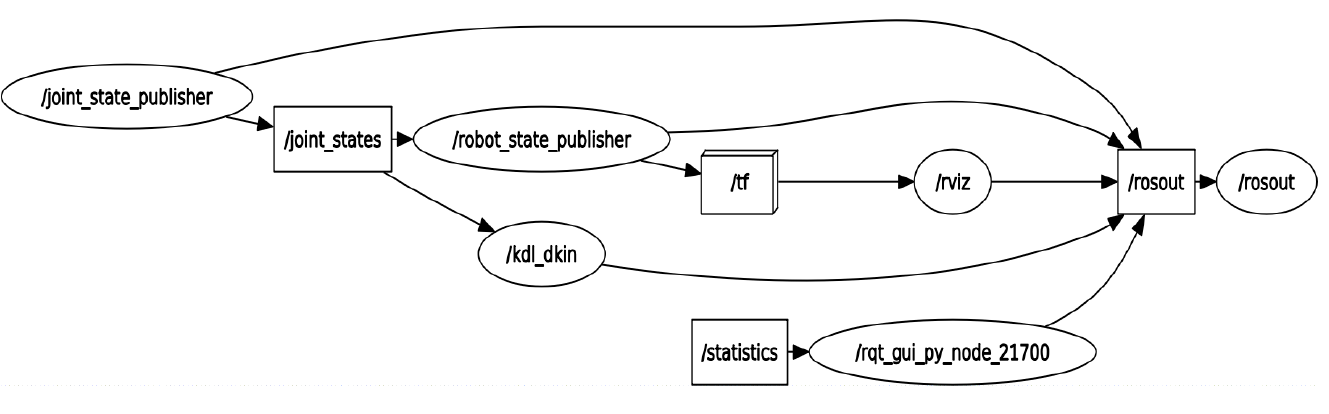
\includegraphics[width=0.8\linewidth]{images/ros_nodes.png}
\caption{Przykładowy schemat komunikacji międzyprocesowej w ROS}
\label{fig:ros_nodes}
\end{figure}

W celu ujednolicenia sposobu definiowania kinematyki, dynamiki i wyglądu robotów oraz udostepnienia możliwości dzielenia się modelami przygotowanymi przez różnych użytkowników zdefiniowano standard opisu URDF (Unified Robotic Description Format) \cite{urdf}. Pliki modeli URDF są to pliki XML, w których definiowane są parametry robota, takie jak:
\begin{itemize}
\item położenia i orientacje początkowe poszczególnych członów i związanych z nimi układów odniesienia,
\item położenia i rodzaje przegubów łączących ze sobą zdefiniowane człony,
\item rozmiary, masy, momenty bezwładności poszczególnych członów,
\item ograniczenia ruchu w przegubach,
\item parametry napedów sterujących ruchem przegubów.
\end{itemize}

\subsubsection{Gazebo}

Gazebo jest darmowym symulatorem dynamiki 3D stworzonym na potrzeby rozwoju robotyki. Umożliwia korzystanie z 4 silników fizycznych: ODE, Bullet, Simbody i DART (domyślnie używany jest ODE). Do renderowania otoczenia i modelu wykorzystuje silnik graficzny OGRE. Dodatkowo Gazebo posiada duży zbiór gotowych, popularnych modeli robotów, które można wykorzystać we własnych projektach, a także pozwala na uruchomienie w zdalnym środowisku lub w chmurze. Ponadto jest łatwo integrowany z pakietem ROS. W niniejszej pracy został użyty do symulowania i sprawdzania poprawności wykonania zadania przed uruchamianiem programu sterującego bezpośrednio na robocie.

\subsubsection{ros\_control}

W celu połączenia oprogramowania symulacyjnego i sterownika robota użyto bibliotekę ros\_control \cite{roscontrol} \cite{roscontrolart}. Jest ona dedykowana do użytku z pakietem ROS i umożliwia szybką implementację oprogramowania sterującego. Biblioteka ta jest szablonem kontrolera robota, który można wykorzystać do własnego projektu. Ponadto posiada zestaw zaimplementowanych, szeroko używanych sterowników ruchu członów robota, które wykorzystują regulator PID. Są to między innymi:

\begin{itemize}
\item velocity\_controllers - sterowanie prędkością/pozycją/mocą na podstawie zadanej prędkości;
\item position\_controllers - sterowanie prędkością/pozycją/mocą na podstawie zadanej pozycji;
\item effort\_controllers - sterowanie prędkością/pozycją/mocą na podstawie zadanej mocy;
\end{itemize}

Dodatkowo biblioteka pozwala na zarządzanie sterownikami w czasie działania za pomocą controller\_managera, który odpowiedzialny jest za nadzorowanie pracy sterowników, inicjalizowanie ich oraz zajmowaniu się sytuacjami konfliktowymi między nimi.

Podstawą działania każdego sterownika pisanego przy użyciu ros\_control jest sprzętowa warstwa abstrakcji (interfejs sprzętowy), która łączy rzeczywistego/symulowanego robota ze sterownikiem programowym. Ta warstwa abstrakcji dostarczona jest poprzez klasę \textit{hardware\_interface::RobotHW} (rysunek \ref{fig:ros_control}). Implementacja sterownika pod konkretnego robota musi dziedziczyć po tej klasie. W ten sposób możliwe jest pisanie oprogramowania, które może zostać w części lub w całości wykorzystane ponownie. Dodatkowo oznacza to, że sterownik napisany z pomocą ros\_control jest niezależny od sprzętu użytego w konstrukcji robota, gdyż zastosowany jest interfejs sprzętowy.

\begin{figure}[hbt!]
\centering
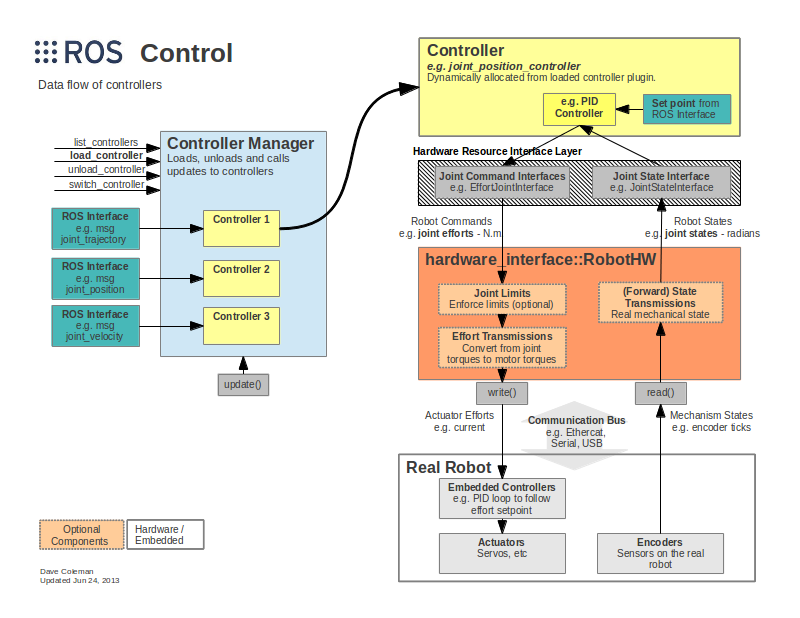
\includegraphics[width=0.8\linewidth]{images/gazebo_ros_control.png}
\caption{Schemat działania sterownika robota opartego o dodatek ros\_control \textit{ (Źródło: \cite{roscontrol}) } }
\label{fig:ros_control}
\end{figure}

Biblioteka ros\_control została w pracy użyta do zaimplementowania sterownika każdego z członów robota (zarówno w symulacji jak i rzeczywistego urządzenia), a także jako warstwa pośrednicząca w komunikacji pomiędzy mikrokontrolerem, a komputerem z uruchomionym oprogramowaniem sterującym i symulacyjnym.

\subsubsection{Spacenav}

Biblioteka spacenav \cite{spacenav} jest darmowym pakietem, który umożliwia użycie myszy 3D firmy 3Dconnexion w połączeniu z ROS. Pakiet oparty jest o darmowe sterowniki do tych urządzeń \cite{spacenavdriver}. Zasada działania biblioteki opiera się o uruchomienie węzła w ROS o nazwie spacenav\_node, który zbiera dane z podłączonego do komputera urządzenia i publikuje je w 4 tematach:

\begin{itemize}
\item spacenav/offset
\item spacenav/rot\_offset
\item spacenav/twist
\item spacenav/joy
\end{itemize}

W ten sposób możliwe jest odczytanie aktualnego wychylenia i obrotu względem osi urządzenia odzcytując dane z powyższych tematów.

\subsubsection{STDPeriph}

Do stworzenia oprogramowania dla mikrokontrolera STM32F407-VET zarządzającego peryferiami robota wykorzystano STDPeriph \cite{stdperiph}. Jest to zbiór bibliotek, które uwalniają użytkownika od konieczności programowania procesorów STM32 stosując tylko zapis bitów do odpowiednich adresów rejestrów. STDPeriph posiada zdefiniowane struktury peryferiów, zmapowane adresy odpowiednich rejestrów dla każdego mikrokontrolera oraz udostępnia API, które ułatwiają inicjalizację i korzystanie z każdej funkcjonalności. Ponadto biblioteki stworzone zostały tak, aby napisany kod mógł zostać użyty bez zmian korzystając z innego mikrokontrolera z tej samej rodziny.

\subsubsection{FreeRTOS}

Aby zapewnić bezpieczne i pewne wykonywanie zadań przez mikrokontroler sterujący manipulatorem zdecydowano się na oparcie oprogramowania o system czasu rzeczywistego. Jednym z takich rozwiązań jest darmowy i szeroko wspierany system FreeRTOS \cite{freertos}, który bardzo dobrze nadaje się do takiego zastosowania ze względu na mały rozmiar i prostotę użytkowania. Jądro zawarte jest w 3 plikach C i jest kompilowane razem z kodem mikrokontrolera. System jest konfigurowalny za pomocą 1 pliku (\textit{FreeRTOSConfig.h}). W ten sposób użytkownik decyduje, które komponenty chce wykorzystać.

Podstawą działania FreeRTOS jest scheduler działający priorytetowo. Każde ze zdefiniowanych zadań ma przypisany priorytet, który decyduje o tym, kiedy zostanie ono wykonane. W przypadku gdy w trakcie działania programu gotowość zgłosi zadanie o priorytecie wyższym nastąpi wywłaszczenie aktualnie wykonywanego zadania na rzecz nowego (zgodnie z \ref{fig:freertos_scheduler}). Jeżeli gotowe są dwa zadania o tym samym priorytecie to będą one kolejkowane na zasadzie podziału czasu. Tak działający scheduler zapewnia terminowość krytycznych zadań. FreeRTOS używa cyklicznego, systemowego przerwania mikrokontrolera (w przypadku STM32 jest to przerwanie SysTick) do wywoływania kodu schedulera, w którym następuje zmiana kontekstu wykonywanego aktualnie zadania (ang. context switching).

\begin{figure}[hbt!]
\centering
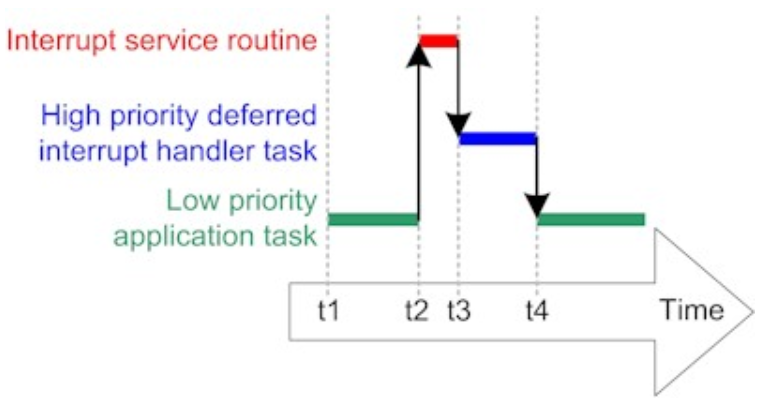
\includegraphics[width=0.8\linewidth]{images/freertos_scheduler.png}
\caption{Schemat kolejności wykonywania zadań we FreeRTOS \textit{ (Źródło: \cite{freertos}) } }
\label{fig:freertos_scheduler}
\end{figure}

Ponadto FreeRTOS oferuje dodatkowe funkcjonalności takie jak:

\begin{itemize}
\item system kolejek (ang. queues) stosowany do komunikacji między zadaniami;
\item możliwość użycia programowego licznika czasu (ang. timer);
\item mutexy, semafory i semafory binarne do zarządzania dostępem do zasobów współdzielonych i synchronizowania zadań
\item mechanizm notyfikacji do synchronizacji wykonywania zadań
\item obsługa błędów poprzez zdefiniowanie przerwań obsługujących przypadki, gdy: brak jest pamięci do stworzenia nowego zadania (przerwanie \textit{vApplicationMallocFailedHook()}), odwołanie do niezdefiniowanego adresu (przerwanie \textit{vApplicationStackOverflowHook()});
\end{itemize}

%%%%%%%%%%%%%%%%%%%%%%%%%%%%%%%%%%%%%%%%
\newpage
\vspace*{1.5 cm}
\section{Specyfikacja systemu}
\vspace{1.5 cm}
W poniższym rozdziale przedstawiono specyfikację systemu sterowania manipulatorem o 6 stopniach swobody. Opisano założenia, przypadki użycia i wyodrębniono agenty systemu.
\subsection{Założenia i wymagania}

\subsubsection{Założenia sprzętowe}
\begin{itemize}
\item Sterowany manipulator ma 6 stopni swobody i wyposażony jest w chwytak dwupalczasty.
\item Efektorami robota są 3 silniki prądu stałego, 1 siłownik i 2 serwa Dynamixel RX-64.
\item Każdy napęd wyposażony jest w enkodery magnetyczne służące do pomiaru prędkości i położeń wałów napędów.
\item Komunikacja z robotem odbywa się poprzez interfejs UART.
\end{itemize}

\subsubsection{Założenia dotyczące systemu}
\begin{itemize}
\item Aby system działał poprawnie wymagana jest obecność manipulatora oraz komputera PC.
\item System pozyskuje dane o ruchu robota na podstawie danych z enkoderów magnetycznych.
\item System pozwala na sterowanie pozycją manipulatora we współrzędnych złączowych lub współrzędnych narzędziowych.
\item Sterowanie robotem może odbywać się poprzez napisanie programu definiującego ruch wykorzystując przygotowany interfejs programistyczny lub za pomocą podłączonego zadajnika.
\item Komendy ruchu mogą być wykonywane przez rzeczywiste urządzenie lub oddzwierciedlone w symulacji dostarczonej ze sterownikiem.
\item Do sterowania ręcznego ruchem manipulatora wymagana jest podłączona do komputera PC mysz 3D.
\item System pozwala na sterowanie chwytakiem podłączonym do manipulatora poprzez jego proste zamknięcie lub otwarcie.
\end{itemize}

\subsection{Przypadki użycia systemu}
Możliwe interakcje użytkownika z systemem  ukazuje diagram przypadków użycia (rysunek \ref{fig:use_cases}):

\begin{figure}[hbt!]
\centering
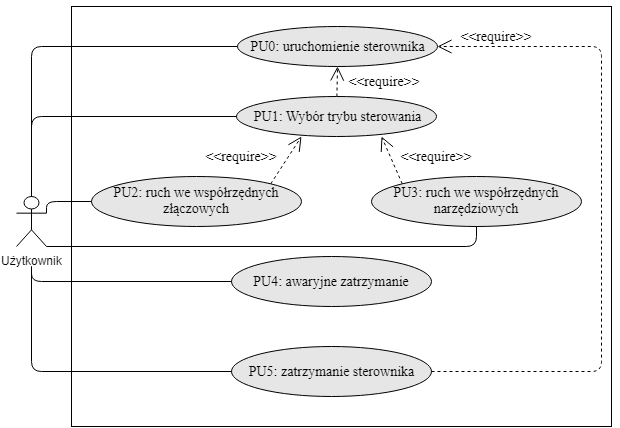
\includegraphics[width=1.0\linewidth]{images/use_cases.png}
\caption{Diagram przypadków użycia systemu }
\label{fig:use_cases}
\end{figure}

W założeniu jedynym aktorem jest użytkownik, który może korzystać ze sterownika za pomocą zadajnika lub używając interfejsu programistycznego. Wyodrębniono 6 przypadków użycia systemu:

\begin{itemize}
\item \textbf{PU0} uruchomienie sterownika - włączenie oprogramowania sterującego na komputerze PC oraz włączenie zasilania manipulatora.
\item \textbf{PU1} wybór trybu sterowania - użytkownik może zdecydować, czy ruch ma być wykonywany w układzie współrzędnych związanym ze złączami, czy z narzędziem.
\item \textbf{PU2} ruch we współrzędnych złączowych - użytkownik po wybraniu trybu pracy we współrzędnych złączowych może definiować ruch manipulatora zadając sterowanie każdemu z członów.
\item \textbf{PU3} ruch we współrzędnych narzędziowych - użytkownik po wybraniu trybu pracy we współrzędnych narzędziowych może definiować ruch manipulatora zadając sterowanie końcówce robota.
\item \textbf{PU4} awaryjne zatrzymanie - użytkownik może w sposób zamierzony lub nie zdecydować o zatrzymaniu pracy robota; manipulator zostanie zatrzymany w przypadku gdy: użytkownik zada taką komendę, nastąpi odłączenie zadajnika w ręcznym trybie pracy, nastąpi przerwanie komunikacji pomiędzy robotem, a komputerem.
\item \textbf{PU5} zatrzymanie sterownika - wyłączenie oprogramowania sterującego na komputerze PC i/lub odłączenie zasilania manipulatora
\end{itemize} 

\subsection{Struktura systemu}

System składa się z dwóch agentów: $a_{robot}$ i $a_{sim}$. Agent $a_{robot}$ jest odpowiedzialny za obsługę peryferiów manipulatora i wykonywanie zadanego ruchu poprzez sterowanie rzeczywistymi napędami oraz otwieranie/zamykanie chwytaka. Stąd agent $a_{robot}$ oczekuje na komendy wydawane przez agenta $a_{sim}$, który decyduje o trybie pracy i sterowaniu ruchem na podstawie otrzymywanych danych.

\begin{figure}[hbt!]
\centering
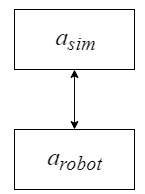
\includegraphics[width=0.2\linewidth]{images/agent_comm.png}
\caption{Komunikacja pomiędzy agentami systemu}
\label{fig:agent_comm}
\end{figure}

Agent $a_{robot}$ posiada jedynie rzeczywiste efektory w postaci napędów sterujących pszczególnymi członami manipulatora ( $E_{robot1}, ...,  E_{robot6}$), a także chwytakiem ($E_{robot7}$). Jego oprogramowanie składa się z jednego podsystemu sterowania oraz efektorów wirtualnych odpowiadających każdemu z efektorów rzeczywistych.

\begin{figure}[hbt!]
\centering
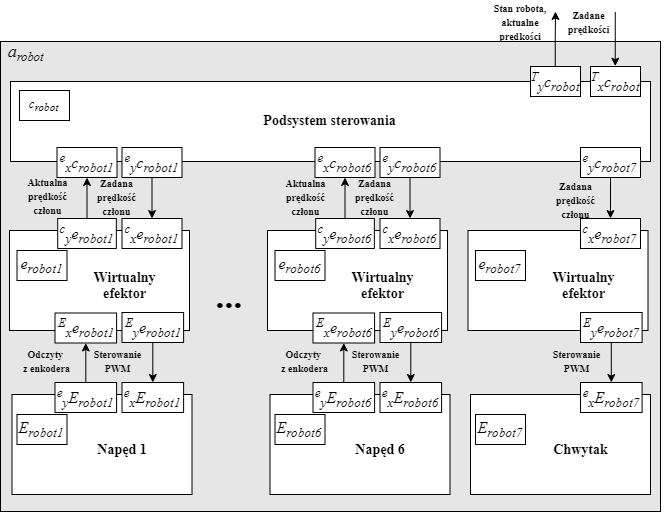
\includegraphics[width=1.0\linewidth]{images/agent_robot.png}
\caption{Schemat agenta $a_{robot}$ }
\label{fig:agent_robot}
\end{figure}

Agent $a_{sim}$ ma wyspecyfikowany jeden rzeczywisty efektor jakim jest ekran monitora, który wizualizuje dane sterowania i symulacje robota. Ponadto agent zawiera dwa reczywiste receptory: klawiaturę, która służy do zmiany stanu manipulatora, a także zadajnik w postaci myszy 3D do ręcznego sterowania robotem. Oprogramowanie agenta składa się z wirtualnych efektorów i recepotrów do obsługi wspomnianych peryferiów, a także z podsystemu sterowania, który jest sterownikiem ruchu manipulatora, obsługuje symulacje oraz wydaje komendy ruchu do agenta $a_{robot}$ na podstawie instrukcji zadanych przez użytkownika.

\begin{figure}[hbt!]
\centering
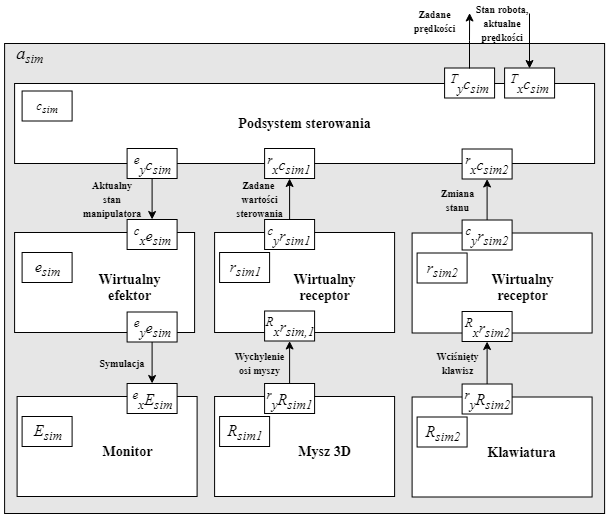
\includegraphics[width=1.0\linewidth]{images/agent_sim.png}
\caption{Schemat agenta $a_{sim}$ }
\label{fig:agent_sim}
\end{figure}

Agenty oraz ich podsystemy przesyłają dane za pośrednictwem buforów wejściowych i wyjściowych. Poniżej przedstawiono tabele \ref{tab:comrobotsim}, która pokazuje komunikację międzyagentową oraz tabele \ref{tab:comrobot} i \ref{tab:comsim} dotyczące komunikacji wewnątrz odpowiednio agentów $a_{robot}$ i $a_{sim}$. 

\begin{table}[htb!] \label{comrobotsim}
\begin{center}
\caption{Komunikacja pomiędzy agentami $a_{robot}$ i $a_{sim}$}
\begin{tabular}{ | l | l | p{6cm} |}
\hline
 Bufor wyjściowy & Bufor wejściowy & Dane \\ 
\hline
 $^T_yc_{sim}$ & $^T_xc_{robot}$ & Komendy sterujące: tryb ruchu i prędkości poszczególnych członów \\ 
\hline
 $^T_yc_{robot}$ & $^T_yc_{sim}$ & Stan robota i aktualne odczyty prędkości członów \\
\hline
\end{tabular}
\end{center}
\end{table}

\begin{table}[htb!]
\label{comrobot}
\begin{center}
\caption{Komunikacja podsystemów agenta $a_{robot}$}
\begin{tabular}{ | l | l | p{6cm} |}
\hline
 Bufor wyjściowy & Bufor wejściowy & Dane \\ 
\hline
 $^e_yE_{robot1..6}$ & $^E_xe_{robot1..6}$ & Odczyty z enkoderów napędów członów 1..6\\ 
\hline
 $^E_ye_{robot1..6}$ & $^e_xE_{robot1..6}$ & Przeliczony sygnał sterujący napędów członów 1..6\\
\hline
 $^c_ye_{robot1..6}$ & $^e_xc_{robot1..6}$ & Przeliczona prędkość członów 1..6 (w [rad/s]) \\
\hline
 $^e_yc_{robot1..6}$ & $^c_xe_{robot1..6}$ & Zadana prędkość członów 1..6 (w [rad/s])\\ 
\hline
 $^E_ye_{robot7}$ & $^e_xE_{robot7}$ & Sygnał sterujący zamykaniem/otwieraniem chwytaka \\
\hline
 $^e_yc_{robot7}$ & $^c_xe_{robot7}$ & Polecenie zamknięcia/otwarcia chwytaka \\ 
\hline
\end{tabular}
\end{center}
\end{table}

\begin{table}[htb!]
\label{comsim}
\begin{center}
\caption{Komunikacja podsystemów agenta $a_{sim}$}
\begin{tabular}{ | l | l | p{6cm} |}
\hline
 Bufor wyjściowy & Bufor wejściowy & Dane \\ 
\hline
 $^E_ye_{sim}$ & $^e_xE_{sim}$ & Symulacja: stan manipulatora \\ 
\hline
 $^e_yc_{sim}$ & $^c_xe_{sim}$ & Aktualny stan manipulatora: prędkości/położenia poszczególnych członów \\
\hline
 $^r_yR_{sim1}$ & $^R_xr_{sim1}$ & Analogowe sygnały wychyleń i rotacji gałki myszy 3D względem każdej z osi \\
\hline
 $^c_yr_{sim1}$ & $^r_xc_{sim1}$ & Przeliczone, procentowe wartości wychyleń i rotacji myszy 3D \\ 
\hline
 $^r_yR_{sim2}$ & $^R_xr_{sim2}$ & Naciśnięty klawisz klawiatury \\
\hline
 $^c_yr_{sim2}$ & $^r_xc_{sim2}$ & Odczytany klawisz i akcja z nim związana \\ 
\hline
\end{tabular}
\end{center}
\end{table}

\subsubsection{Podsystem sterowania $c_{robot}$}
W podsystemie sterowania wyodrębniono 6 stanów. Na początku odbywa się inicjalizacja peryferiów robota, synchronizacja napędów i ich zatrzymanie w stanie \textit{INIT}. Jeżeli wszystkie peryferia zostaną zainicjalizowane poprawnie i nie ma potrzeby ponownego ich uruchamiania lub uśpienia kontrolera (\textbf{~r\_s}) wtedy następuje przejście do stanu \textit{IDLE}. W tym stanie system oczekuje na komunikację z agentem $a_{sim}$ jednocześnie utrzymując zadane prędkości zerowe na silnikach (zatrzymanie). W przypadku gdy następuje potrzeba ponownego ustawienia peryferiów (\textbf{r\_s}) system przechodzi do stanu \textit{RESET}, w którym następuje uśpienie, a w momencie gdy możliwa jest dalsza praca wykonywana jest reinicjalizacja i powrót do stanu \textit{IDLE}. Jeżeli w stanie \textit{IDLE} nawiązana zostanie komunikacja (\textbf{e\_s}) to w zależności od trybu pracy (\textbf{j\_m} lub \textbf{t\_m}) wykonywane jest zadane sterowanie odpowiednio we współrzędnych złączowych (stan \textit{JOINT\_MODE}) lub narzędziowych (stan \textit{TOOL\_MODE}. Każda zmiana trybu pracy lub utrata komunikacji powoduje zatrzymanie napędów (stan \textit{STOP}) i powrót do stanu \textit{IDLE}.

\begin{figure}[hbt!]
\centering
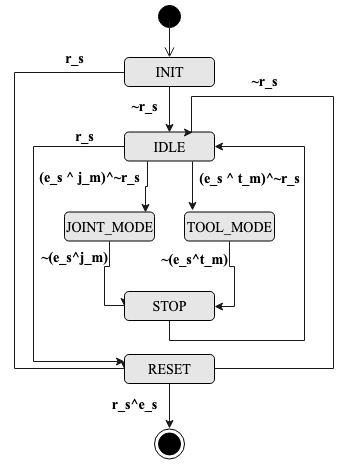
\includegraphics[width=0.6\linewidth]{images/state_robot.png}
\caption{Automat skończony podsystemu sterowania $c_{robot}$ }
\label{fig:state_robot}
\end{figure}

\begin{table}[htb!]
\label{behaviour_robot}
\begin{center}
\caption{Zachowania podsystemu sterowania $c_{robot}$ i odpowiadające im stany}
\begin{tabular}{ | l | l | l |}
\hline
 Stan & Zachowanie & Opis \\ 
\hline
 $^cS_{robot,0}$ & $^cB_{robot,0}$ & INIT: Inicjalizacja  \\ 
\hline
 $^cS_{robot,1}$ & $^cB_{robot,1}$ & IDLE: Bezczynność \\
\hline
 $^cS_{robot,2}$ & $^cB_{robot,2}$ & JOINT\_MODE: Sterowanie w trybie złączowym \\
\hline
 $^cS_{robot,3}$ & $^cB_{robot,3}$ & TOOL\_MODE: Sterowanie w trybie narzędziowym \\
\hline
 $^cS_{robot,4}$ & $^cB_{robot,4}$ & STOP: Zatrzymanie \\
\hline
 $^cS_{robot,5}$ & $^cB_{robot,5}$ & RESET: Reinicjalizacja \\
\hline
\end{tabular}
\end{center}
\end{table}

Poniżej przedstawiono opis zachowań podsystemu sterowania $c_{robot}$:

\paragraph{Inicjalizacja ($^cB_{robot,0}$)}

\begin{itemize}
\item warunek początkowy: 
\item warunek końcowy:
\item funkcja przejścia:
\end{itemize}

\paragraph{Bezczynność ($^cB_{robot,1}$)}

\begin{itemize}
\item warunek początkowy: 
\item warunek końcowy:
\item funkcja przejścia:
\end{itemize}

\paragraph{Sterowanie w trybie złączowym ($^cB_{robot,2}$)}

\begin{itemize}
\item warunek początkowy: 
\item warunek końcowy:
\item funkcja przejścia:
\end{itemize}

\paragraph{Sterowanie w trybie narzędziowym ($^cB_{robot,3}$)}

\begin{itemize}
\item warunek początkowy: 
\item warunek końcowy:
\item funkcja przejścia:
\end{itemize}

\paragraph{Zatrzymanie ($^cB_{robot,4}$)}

\begin{itemize}
\item warunek początkowy: 
\item warunek końcowy:
\item funkcja przejścia:
\end{itemize}

\paragraph{Reset ($^cB_{robot,5}$)}

\begin{itemize}
\item warunek początkowy: 
\item warunek końcowy:
\item funkcja przejścia:
\end{itemize}

\subsubsection{Rzeczywiste efektory $E_{robot1..6}$}

\subsubsection{Wirtualne efektory $e_{robot1..6}$}

\subsubsection{Rzeczywisty efektor $E_{robot7}$}

\subsubsection{Wirtualny efektor $e_{robot7}$}

\subsubsection{Podsystem sterowania $c_{sim}$}

\subsubsection{Rzeczywisty receptor $R_{sim1}$}

\subsubsection{Wirtualny receptor $r_{sim1}$}

\subsubsection{Rzeczywisty receptor $R_{sim2}$}

\subsubsection{Wirtualny receptor $r_{sim2}$}

%%%%%%%%%%%%%%%%%%%%%%%%%%%%%%%%%%%%%%%%

%%%%%%%%%%%%%%%%%%%%%%%%%%%%%%%%%%%%%%%%
\newpage
\vspace*{1.5 cm}
\section{Oprogramowanie kontrolera}
\vspace{1.5 cm}
%TODO

%%%%%%%%%%%%%%%%%%%%%%%%%%%%%%%%%%%%%%%%

%%%%%%%%%%%%%%%%%%%%%%%%%%%%%%%%%%%%%%%%
\newpage
\vspace*{1.5 cm}
\section{Sterownik i symulacja}
\vspace{1.5 cm}
%TODO

%%%%%%%%%%%%%%%%%%%%%%%%%%%%%%%%%%%%%%%%

\newpage
\vspace*{1.5 cm}
\section{Weryfikacja}
\vspace{1.5 cm}
%TODO
\subsection{Metody generowania trajektorii}

Oprogramowanie sterujące robotem powinno pozwalać na zaprogramowanie go, aby mógł podążać wyznaczoną ścieżką. Użytkownik zadaje 
\subsubsection{Interpolacja liniowa}
%TODO
\subsubsection{Interpolacja wielomianami sklejanymi}
%TODO


%%%%%%%%%%%%%%%%%%%%%%%%%%%%%%%%%%%%%%%%
\newpage
\vspace*{1.5 cm}
\section{Opracowanie wyników}  \label{wyniki}
\vspace{3.0 cm}
%TODO
\vspace{1.0 cm}

%%%%%%%%%%%%%%%%%%%%%%%%%%%%%%%%%%%%%%%%
\newpage
\vspace*{1.5 cm}
\section{Podsumowanie}
\vspace{3.0 cm}

%%%%%%%%%%%%%%%%%%%%%%%%%%%%%%%%%%%%%%%%
\newpage
\section*{DODATEK A. Zawartość płyty CD}
\addcontentsline{toc}{section}{DODATEK A. ZAWARTOŚĆ PŁYTY CD}
\vspace{3.0 cm}

%%%%%%%%%%%%%%%%%%%%%%%%%%%%%%%%%%%%%%%%
\newpage
% Bibliografia
\section*{}
\addcontentsline{toc}{section}{BIBLIOGRAFIA}
\printbibliography

%%%%%%%%%%%%%%%%%%%%%%%%%%%%%%%%%%%%%%%%
\newpage
\section*{Wykaz symboli i skrótów}
\addcontentsline{toc}{section}{WYKAZ SYMBOLI I SKRÓTÓW}

\DTLnewdb{acronyms}
\addacronym{ROS}{Robot Operating System}
\addacronym{RTOS}{Real Time Operating System}
\addacronym{SysML}{System Modelling Language}
\addacronym{STDPeriph}{Standard Peripheral Libraries}
\addacronym{ISO}{International Organisation for Standarization}
\addacronym{KRL}{KUKA Robot Language}
\addacronym{IMU}{Inertial Measurement Unit}
\addacronym{URC}{University Rover Challenge}
\addacronym{UML}{Unified Modelling Language}
\addacronym{API}{Application Programming Interface}
% Sort the database
\DTLsort*{Acronym}{acronyms}

%Show acronyms
\begin{itemize}[label={}, leftmargin=*]
\DTLforeach*{acronyms}{\thisAcronym=Acronym,\thisDesc=Description}
   {\item \textbf{\thisAcronym}   \thisDesc}
\end{itemize}

%%%%%%%%%%%%%%%%%%%%%%%%%%%%%%%%%%%%%%%%
\newpage
\addcontentsline{toc}{section}{SPIS RYSUNKÓW}
\listoffigures

%%%%%%%%%%%%%%%%%%%%%%%%%%%%%%%%%%%%%%%%
\newpage
\addcontentsline{toc}{section}{SPIS TABLIC}
\listoftables
\end{document}